\documentclass[ngerman]{gdb-aufgabenblatt}
\usepackage{paralist}

\renewcommand{\Aufgabenblatt}{2}
\renewcommand{\Ausgabedatum}{Mi. 30.10.2013}
\renewcommand{\Abgabedatum}{Do. 14.11.2013}
\renewcommand{\Gruppe}{Dammer, Teuteberg, Wilhelm}


\begin{document}


\section{Informationsmodellierung: Erstellung eines ER-Modells}

\centerline{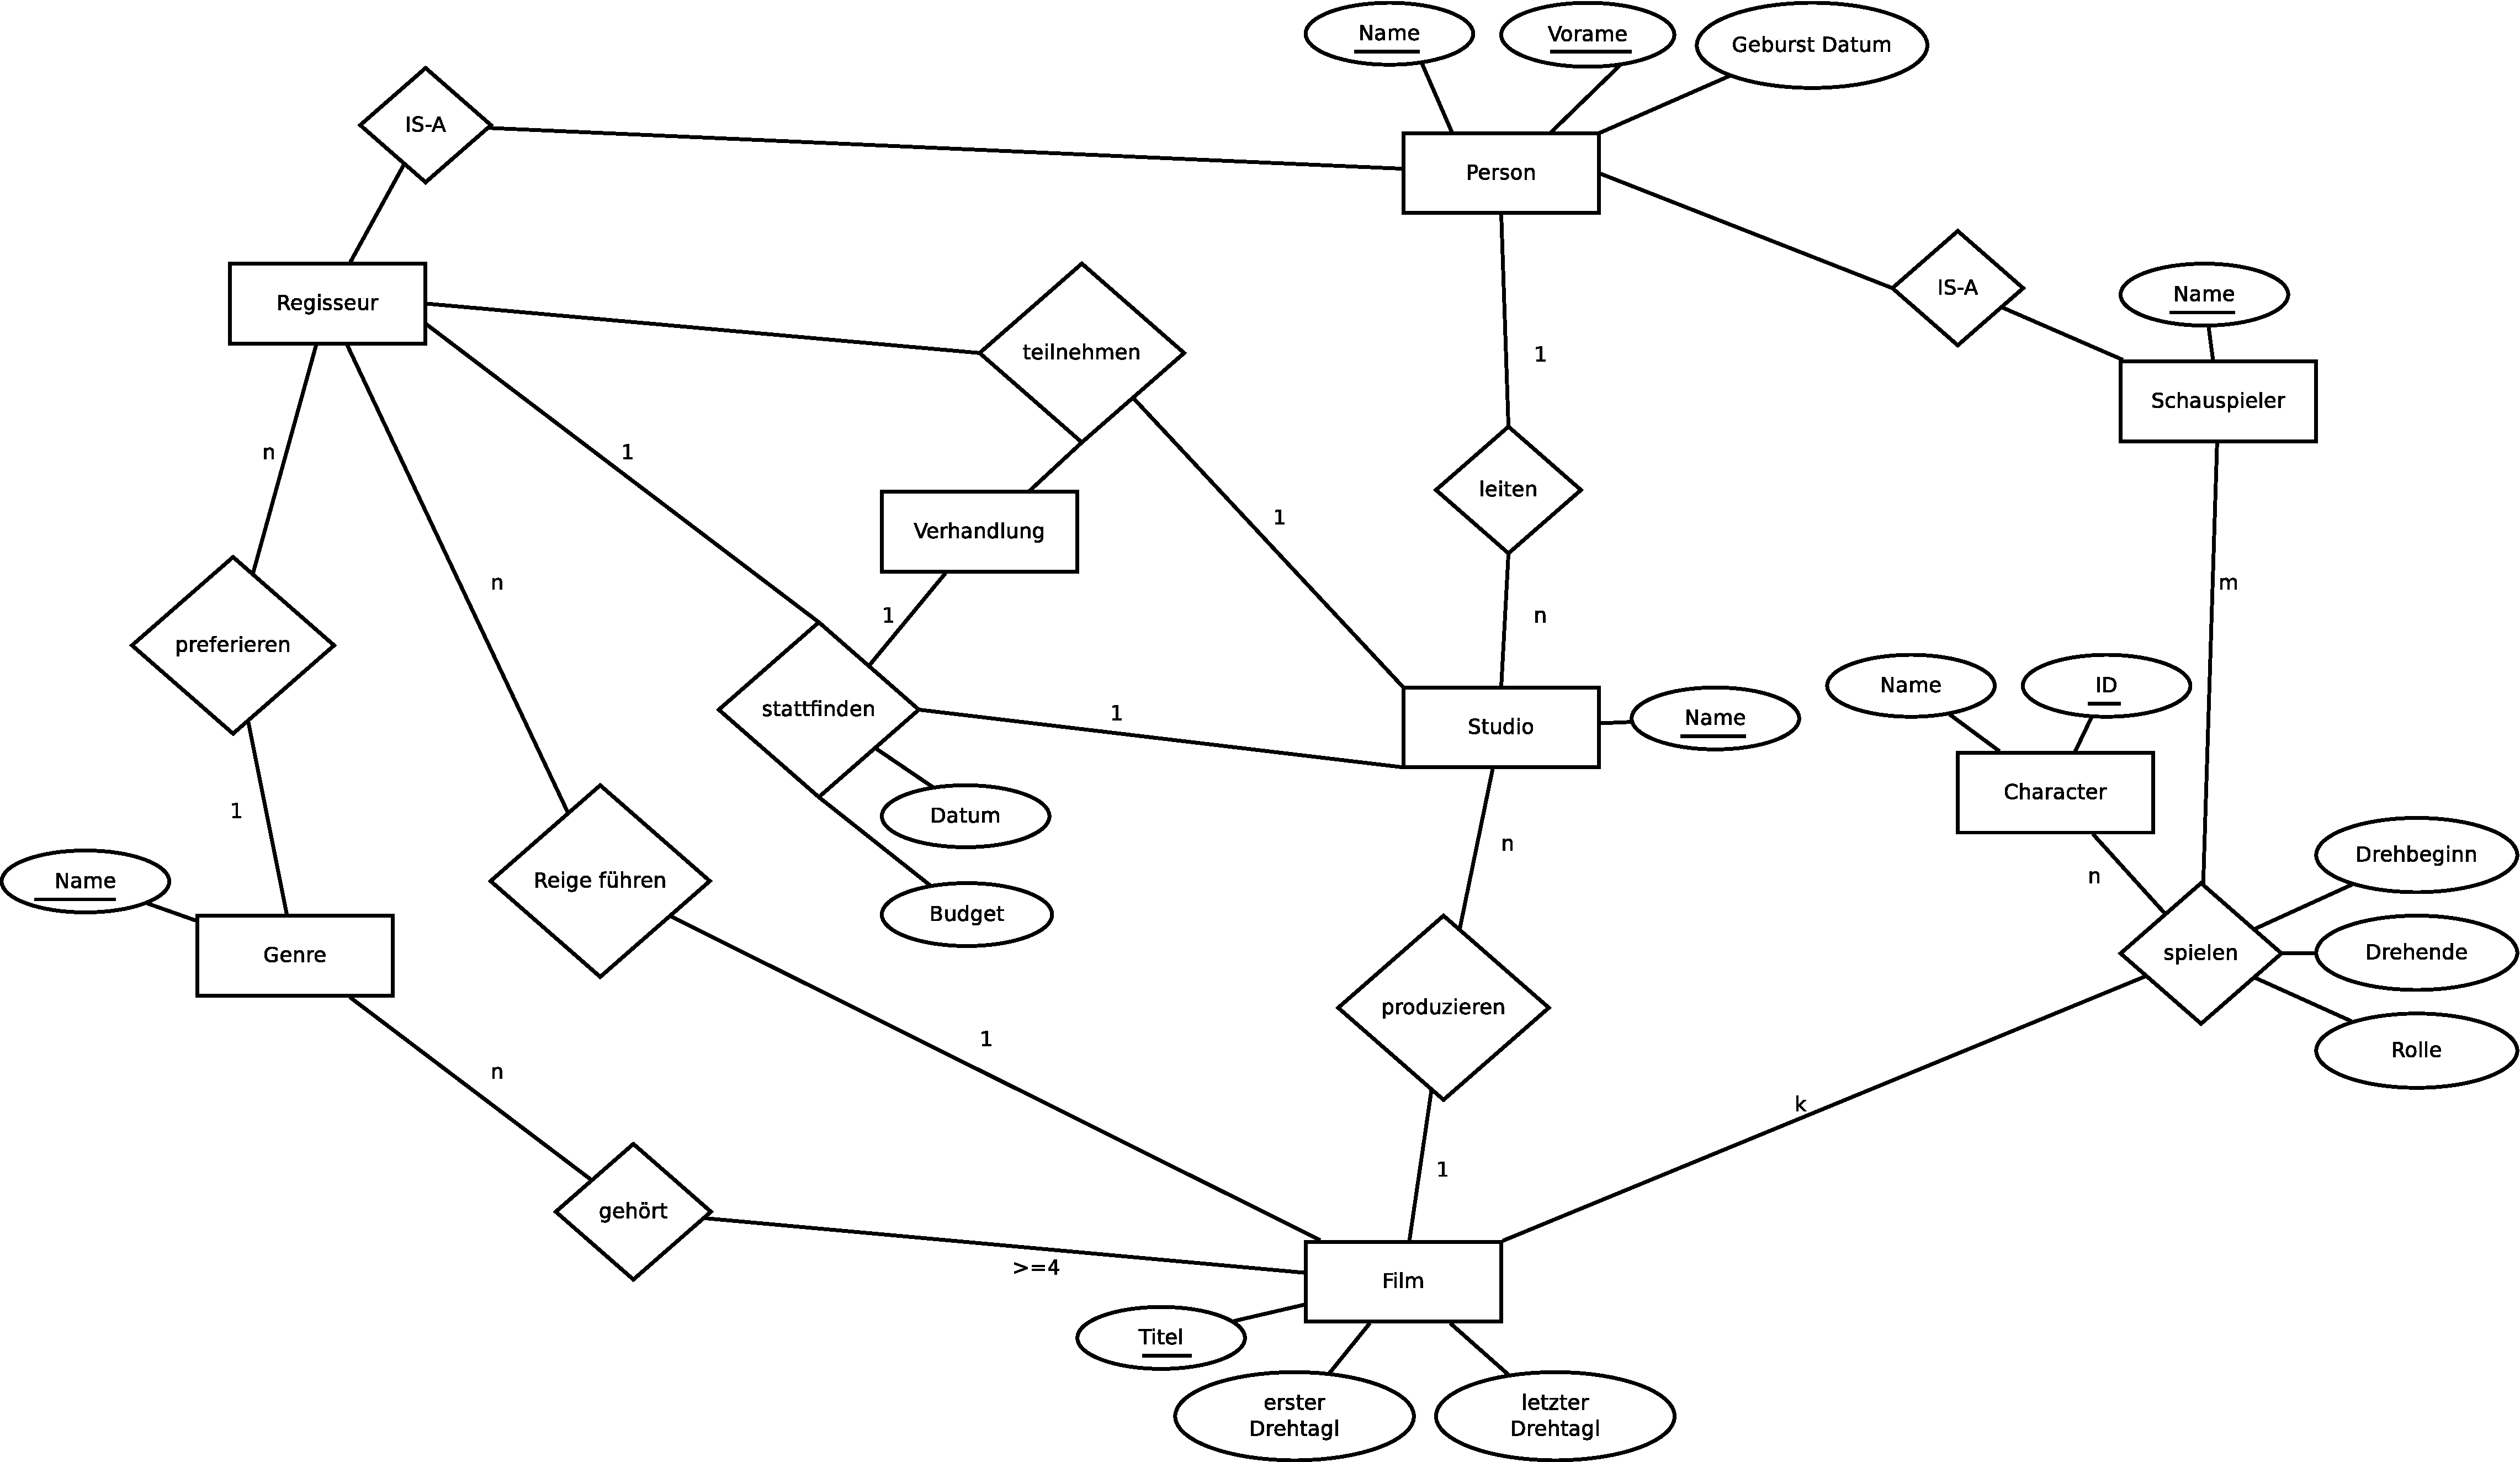
\includegraphics[scale=0.2]{Aufgabe1HA2.pdf}} \par 
\begin{compactenum}[(i)]
	\item Ein Schauspieler kann nicht eine Rolle im Film spielen, falls der letzte Drehtag des Films fr\"uher ist als der Drehbeginn des Schauspielers. \\
	\item Der Regisseur kann nicht den Film produzieren, dessen letzter Drehtag fr\"uher ist als das Geburtsdatum des Regisseurs.\\
\end{compactenum}


\section{Informationsmodellierung: Beschreibung von ER-Modellen}

\begin{compactenum}[(a)]
	\item Bin\"are Relationship. Beziehungstyp: 1:n\\ 
	Der Entitytyp  \textit{Student} hat zwei Attribute \textit{MatrNr} und \textit{Name}. Das Attribut \textit{MatrNr} ist der Schl\"ussel, der einen Studenten eindeutig identifiziert.\\
	Der Entitytyp \textit{Studiengang} hat nur ein Attribut \textit{Name}, das gleichzeitig der Schl\"ussel ist und eindeutig einen Studiengang identifiziert.\\
	Ein Student darf sich nur in einem Studiengang immatrikulieren.\\
	In einem Studiengang k\"onnen beliebig viele (n) Studenten immatrikuliert sein.\\
	\item Existenzabh\"angigkeit\\
	Der Entitytyp \textit{H\"orsaal} mit den Attributen \textit{Name} und \textit{Pl\"atze} ist existenzabh\"angig vom Entitytyp \textit{Universit\"at} mit dem Attribut \textit{Name} (Schl\"ussel).\\ 
	Alle H\"ors\"ale in derselben Universit\"at haben einen eindeutigen Namen, aber verschiedene Universit\"aten k\"onnen durchaus H\"ors\"ale mit demselben Namen haben. Demnach werden H\"ors\"ale global eindeutig durch den Universit\"atsnamen und den H\"orsaalsnamen identifiziert.\\
	Ein H\"orsaal geh\"ort genau zu einer bestimmten Universit\"at.\\
	Eine Universit\"at hat mindestens einen bis beliebig viele H\"ors\"ale.\\
	\item Tern\"are Relationship. Beziehungstyp: m:n:o\\
	Jeder Auftrag kann mit mehreren Reparaturtypen zusammenh\"angen und dabei k\"onnen mehrere Ersatzteile benutzt werden.\\
	Zu jedem Reparaturtyp k\"onnen mehrere Auftr\"age angenommen werden, die unterschiedliche Ersatzteile ben\"otigen.\\
	Jeder Auftrag hat ein \textit{Datum} und eine eindeutige \textit{ANR}(Schl\"ussel).\\
	Ein Reparaturtyp wird durch die \textit{Art}(Schl\"ussel) und den jeweiligen \textit{Festpreis} beschrieben.\\
	Ein Ersatzteil ist durch das eindeutige \textit{Automodell} und den genauen \textit{Namen} und den jeweiligen \textit{Preis} beschrieben, wobei die Kombination aus  \textit{Automodell} und  \textit{Name} den Schl\"ussel darstellt.\\
	Bei der Relationship \textit{Reparatur} spielen au"serdem die Uhrzeit und das Datum eine Rolle. \\
	\item Die reflexive Relationship \textit{Fussballspiel} setzt zwei Entit\"aten des Entitytyps \textit{Mannschaft} zu einander in Beziehung.\\
	Jedes Fussballspiel wird von zwei Entit\"aten des Typs \textit{Mannschaft} gespielt, wobei es sein kann das einzelne Entit\"aten nie bis beliebig oft an Fu"sballspielen beteiligt sind. Au"serdem sind an jedem Fu"sballspiel noch die Entity-Typen \textit{Stadion} und \textit{Schiedsrichter} beteiligt. Auch f\"ur die beiden Entity-Typen k\"onnen die Entit\"aten jeweils 0 bis beliebig oft an einem Fu"sballspiel teilnehmen.\\
	 
\end {compactenum}


\section{Schl\"usselkandidaten}
\begin{compactenum}[(a)]
	\item Ein Schl\"usselkandidat muss eindeutig und minimal sein. Die Eigenschaft "'eindeutig"' bedeutet, dass ein Schl\"usselkandidat eine Entit\"at zweifelsfrei identifizieren kann. Im Bespiel der Tabelle w\"are ein eindeutiger Kandidat die Telefonnummer, da diese f\"ur alle Tupel eindeutig ist. \\
	Die Eigenschaft "'minimal"' bedeutet, dass der gew\"ahlte Schl\"usselkandidat der kleinstm\"ogliche sein muss. Eine Kombination aus Vor- und Nachname in der Tabelle w\"urde zwar die Eigenschaft "'eindeutig"' eines Schl\"usselkandidaten erf\"ullen. Da es aber auch die Telefonnummer als Schl\"usselkandidaten gibt und dabei keine Kombination mit einem weiteren Attribut n\"otig ist, w\"are die Kombination aus Vor- und Nachname f\"ur die Tabelle also nicht minimal. \\
	M\"ogliche Schl\"usselkandidaten sind also z.B. die Telefonnummer oder die Kombination aus Vorname und Geburtsdatum. \\
	Die Kombination von Vorname und Hausnummer ist kein geeigneter Schl\"usselkandidat, da sie nicht eindeutig ist. Es gibt zweimal die Kombination von Frida und 8. \\
	\item Wenn die Liste mit beliebig vielen Eintr\"agen gef\"ullt w\"are, w\"urden sich die vorhandenen Attribute nicht unbedingt als Schl\"usselkandidaten eignen, da Wiederholungen von Attributen oder auch Attribut-Kombinationen nicht ausgeschlossen werden k\"onnen. So k\"onnte es z.B. sein, dass die Telefonnummer als Schl\"usselkandidat gew\"ahlt wurde. Es k\"onnte durchaus sein, dass in der Liste eine weitere Person mit der gleichen Telefonnummer auftaucht (z.B. wegen gleicher Wohnung). Damit w\"aren diese Personen nicht mehr eindeutig identifizierbar.\\
	Eine L\"osung w\"are das Einf\"uhren eines eindeutigen Attributs, wie beispielsweise einer Personennummer, bei der man sicher sein kann, dass diese nicht wiederholt eingesetzt werden kann. Das w\"are dann ein geeigneter Schl\"usselkandidat.
\end{compactenum}

\end{document}